
\begin{figure}[tbh]
\def\oc{0.6}
\begin{tikzpicture}[scale=0.55,
 locnode/.style = {draw,inner sep=0.5mm, circle,fill=black!10, blur shadow={shadow blur steps=3}},
 tlocnode/.style = {draw,inner sep=0.5mm, circle,fill=green!20, blur shadow={shadow blur steps=3}},
 scale=2, font=\scriptsize]


\node[locnode] (A) at (0,0) {A};
\node[locnode] (B) at (0.6+\oc/2,0.8) {B};
\node[locnode] (C) at (1.4+\oc*1.5,0.8) {C};
\node[locnode] (D) at (1+\oc,0) {D};
\node[tlocnode] (E) at (2+2*\oc,0) {E};


\node[inner sep=0pt] (drone) at (-0.8,0)
    {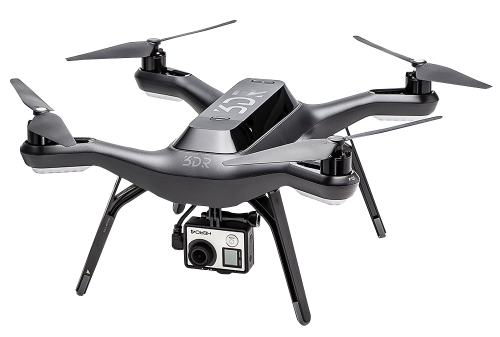
\includegraphics[width=.07\textwidth]{figures/drone.png}};

\filldraw[fill=black!40!white, draw=black, rounded corners] (0.6+\oc,0.25) rectangle (1.4+\oc,0.55);

\begin{scope}[> = stealth,  ->,black,thick, every node/.style = {black,right,align=center}]
\draw (A) edge node[left, xshift=-5pt, yshift=5pt]       {d=10m\\pc=0}     (B);
%\draw (B) edge node       {}     (A);

\draw (B) edge node[yshift=10pt,xshift=-18pt]       {d=8m, pc=0}  (C);
%\draw (C) edge node       {}     (B);
 
\draw (C) edge node[right,xshift=5pt, yshift=5pt]       {d=10m\\pc=0}  (E);
%\draw (E) edge node       {}     (C);

\draw (A) edge node[yshift=-10pt,xshift=-20pt]       {d=10m, pc=0.5}  (D);
%\draw (D) edge node       {}     (A);

\draw (D) edge node[yshift=-10pt,xshift=-20pt]       {d=10m, pc=0}  (E);
%\draw (E) edge node       {}     (D);


\end{scope}
\end{tikzpicture}
%\vspace{-0.3cm}
\caption{Simple mobile robotics scenario}
\label{fig:robotscenario}
%\vspace{-0.3cm}
\end{figure}